% SECTION 3.3: SPECIAL TRIANGLES AND ANGLES IN STANDARD POSITION

\documentclass[aspectratio=169]{beamer}
\usepackage{amsmath}
\usepackage{amssymb}
\usepackage{graphicx}
\usepackage{tcolorbox}
\usepackage{booktabs}
\usepackage{colortbl}
\usepackage{xcolor}
\usepackage{tikz}
\usetikzlibrary{angles,quotes}
\usepackage[utf8]{inputenc}

% Custom colors
\definecolor{primary}{RGB}{41, 128, 185}
\definecolor{secondary}{RGB}{52, 152, 219}
\definecolor{accent}{RGB}{231, 76, 60}
\definecolor{lightgray}{RGB}{236, 240, 241}

% Theme customization
\usetheme{Madrid}
\usecolortheme{whale}
\setbeamercolor{structure}{fg=primary}
\setbeamercolor{background canvas}{bg=white}
\setbeamercolor{normal text}{fg=black}

% Title page info
\title{Pre-Calculus 11}
\subtitle{Lesson 3.3: Special Triangles and Angles in Standard Position}
\author{Created by Yi-Chen Lin}
\date{\today}

\begin{document}

\begin{frame}
    \titlepage
\end{frame}

% I) REVIEW: EQUILATERAL, ISOSCELES, AND RIGHT TRIANGLES
\begin{frame}{Review: Equilateral, Isosceles, and Right Triangles}
    \begin{tcolorbox}[colback=lightgray,colframe=primary,title=Triangle Types]
        \footnotesize
        \begin{itemize}
            \item \textbf{Equilateral Triangle}: All 3 sides and all angles are equal ($60^\circ$ each)
            \item \textbf{Isosceles Triangle}: Two sides are equal, two angles are equal
            \item \textbf{Isosceles Right Triangle}: Both isosceles and right triangle ($45^\circ$, $45^\circ$, $90^\circ$)
        \end{itemize}
    \end{tcolorbox}
    \vspace{0.5em}
    \begin{columns}
        \column{0.33\textwidth}
        \centering
        \textbf{Equilateral}
        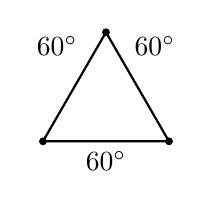
\begin{tikzpicture}[scale=0.8]
            \draw[thick] (0,0) -- (2,0) -- (1,1.732) -- cycle;
            \foreach \x in {(0,0),(2,0),(1,1.732)} \filldraw[black] \x circle (1.5pt);
            \node[below] at (1,0) {$60^\circ$};
            \node[above left] at (0.7,1.2) {$60^\circ$};
            \node[above right] at (1.3,1.2) {$60^\circ$};
        \end{tikzpicture}
        \column{0.33\textwidth}
        \centering
        \textbf{Isosceles}
        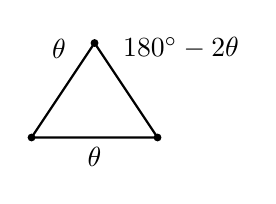
\begin{tikzpicture}[scale=0.8]
            \draw[thick] (0,0) -- (2,0) -- (1,1.5) -- cycle;
            \foreach \x in {(0,0),(2,0),(1,1.5)} \filldraw[black] \x circle (1.5pt);
            \node[below] at (1,0) {$\theta$};
            \node[above left] at (0.7,1.1) {$\theta$};
            \node[above right] at (1.3,1.1) {$180^\circ-2\theta$};
        \end{tikzpicture}
        \column{0.33\textwidth}
        \centering
        \textbf{Isosceles Right}
        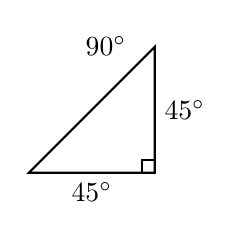
\begin{tikzpicture}[scale=0.8]
            \draw[thick] (0,0) -- (2,0) -- (2,2) -- cycle;
            \draw[thick] (1.8,0) -- (1.8,0.2) -- (2,0.2);
            \node[below] at (1,0) {$45^\circ$};
            \node[right] at (2,1) {$45^\circ$};
            \node[above left] at (1.7,1.7) {$90^\circ$};
        \end{tikzpicture}
    \end{columns}
\end{frame}

% II) WHAT ARE SPECIAL TRIANGLES?
\begin{frame}{What are Special Triangles?}
    \begin{tcolorbox}[colback=lightgray,colframe=primary,title=Special Triangles]
        \footnotesize
        \begin{itemize}
            \item \textbf{Two types:}
            \begin{itemize}
                \item $30^\circ$-$60^\circ$-$90^\circ$ triangle (from equilateral)
                \item $45^\circ$-$45^\circ$-$90^\circ$ triangle (isosceles right)
            \end{itemize}
            \item The side ratios of these triangles are used to find exact values of sine, cosine, and tangent for $30^\circ$, $45^\circ$, $60^\circ$
        \end{itemize}
    \end{tcolorbox}
\end{frame}

% III) 30-60-90 TRIANGLE: DIAGRAM AND RATIOS
\begin{frame}{30-60-90 Triangle: Diagram and Ratios}
    \begin{columns}
        \column{0.5\textwidth}
        \begin{tcolorbox}[colback=lightgray,colframe=primary,title=30-60-90 Triangle]
            \footnotesize
            \begin{itemize}
                \item Start with an equilateral triangle (all sides $k$)
                \item Cut in half to get a $30^\circ$-$60^\circ$-$90^\circ$ triangle
                \item Side ratios: $1 : \sqrt{3} : 2$
            \end{itemize}
        \end{tcolorbox}
        \column{0.5\textwidth}
        \centering
        % Clear, upright, color-labeled triangle
        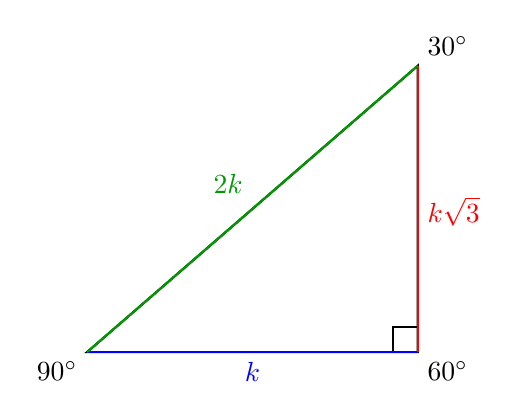
\begin{tikzpicture}[scale=2.1]
            % Right triangle
            \draw[thick] (0,0) -- (2,0) -- (2,1.732) -- cycle;
            % Right angle box
            \draw[thick] (1.85,0) -- (1.85,0.15) -- (2,0.15);
            % Sides
            \draw[thick,blue] (0,0) -- (2,0); % base
            \draw[thick,red] (2,0) -- (2,1.732); % height
            \draw[thick,green!60!black] (0,0) -- (2,1.732); % hypotenuse
            % Side labels
            \node[blue,below] at (1,0) {$k$};
            \node[red,right] at (2,0.85) {$k\sqrt{3}$};
            \node[green!60!black,above left] at (1,0.9) {$2k$};
            % Angles
            \node[below left] at (0,0) {$90^\circ$};
            \node[above right] at (2,1.732) {$30^\circ$};
            \node[below right] at (2,0) {$60^\circ$};
        \end{tikzpicture}
    \end{columns}
\end{frame}

% IV) 45-45-90 TRIANGLE: DIAGRAM AND RATIOS
\begin{frame}{45-45-90 Triangle: Diagram and Ratios}
    \begin{columns}
        \column{0.6\textwidth}
        \begin{tcolorbox}[colback=lightgray,colframe=primary,title=45-45-90 Triangle]
            \footnotesize
            \begin{itemize}
                \item Isosceles right triangle: two sides equal, one $90^\circ$ angle
                \item Side ratios: $1 : 1 : \sqrt{2}$
            \end{itemize}
        \end{tcolorbox}
        \column{0.4\textwidth}
        \centering
        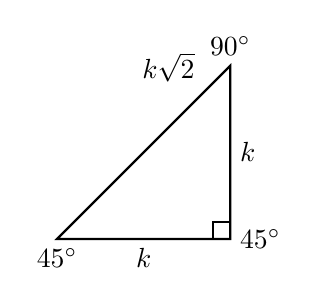
\begin{tikzpicture}[scale=1.1]
            \draw[thick] (0,0) -- (2,0) -- (2,2) -- cycle;
            \draw[thick] (1.8,0) -- (1.8,0.2) -- (2,0.2);
            \node[below] at (1,0) {$k$};
            \node[right] at (2,1) {$k$};
            \node[above left] at (1.7,1.7) {$k\sqrt{2}$};
            \node[below] at (0,0) {$45^\circ$};
            \node[right] at (2,0) {$45^\circ$};
            \node[above] at (2,2) {$90^\circ$};
        \end{tikzpicture}
    \end{columns}
\end{frame}

% V) EXACT VALUES USING SPECIAL TRIANGLES
\begin{frame}{Exact Trig Values Using Special Triangles}
    \begin{tcolorbox}[colback=lightgray,colframe=primary,title=Exact Values]
        \footnotesize
        \begin{itemize}
            \item Use the side ratios to find exact values:
            \begin{align*}
                \sin 30^\circ &= \frac{1}{2} & \cos 30^\circ &= \frac{\sqrt{3}}{2} & \tan 30^\circ &= \frac{1}{\sqrt{3}} \\
                \sin 45^\circ &= \frac{1}{\sqrt{2}} & \cos 45^\circ &= \frac{1}{\sqrt{2}} & \tan 45^\circ &= 1 \\
                \sin 60^\circ &= \frac{\sqrt{3}}{2} & \cos 60^\circ &= \frac{1}{2} & \tan 60^\circ &= \sqrt{3}
            \end{align*}
        \end{itemize}
    \end{tcolorbox}
\end{frame}

% VI) USING SPECIAL TRIANGLES FOR REFERENCE ANGLES
\begin{frame}{Using Special Triangles for Reference Angles}
    \begin{tcolorbox}[colback=lightgray,colframe=primary,title=Reference Angles]
        \footnotesize
        \begin{itemize}
            \item If an angle has a reference angle of $30^\circ$, $45^\circ$, or $60^\circ$, use special triangles to find exact trig values
            \item Example: $\sin 330^\circ$, $\cos 225^\circ$, $\tan 120^\circ$
        \end{itemize}
    \end{tcolorbox}
    \vspace{0.5em}
    \begin{columns}
        \column{0.5\textwidth}
        \centering
        \textbf{Example: $\sin 330^\circ$}
        \begin{tikzpicture}[scale=1.1]
            \draw[thick,->] (-1.1,0) -- (1.1,0) node[right] {$0^\circ$/$360^\circ$};
            \draw[thick,->] (0,-1.1) -- (0,1.1) node[above] {$90^\circ$};
            \draw[thick] (-1,0) -- (-1.1,0) node[left] {$180^\circ$};
            \draw[thick] (0,-1) -- (0,-1.1) node[below] {$270^\circ$};
        \end{tikzpicture}
        \column{0.5\textwidth}
        \centering
        \textbf{Example: $\cos 225^\circ$}
        \begin{tikzpicture}[scale=1.1]
            \draw[thick,->] (-1.1,0) -- (1.1,0) node[right] {$0^\circ$/$360^\circ$};
            \draw[thick,->] (0,-1.1) -- (0,1.1) node[above] {$90^\circ$};
            \draw[thick] (-1,0) -- (-1.1,0) node[left] {$180^\circ$};
            \draw[thick] (0,-1) -- (0,-1.1) node[below] {$270^\circ$};
        \end{tikzpicture}
    \end{columns}
\end{frame}

% VII) PRACTICE PROBLEMS
\begin{frame}{Practice: Special Triangles}
    \begin{tcolorbox}[colback=lightgray,colframe=accent,title=Practice]
        \footnotesize
        Use special triangles to find the exact value of each:
        \begin{itemize}
            \item $\sin 120^\circ$
            \item $\cos 300^\circ$
            \item $\tan 135^\circ$
            \item $\sin 225^\circ$
        \end{itemize}
    \end{tcolorbox}
\end{frame}

\begin{frame}{Practice: Draw and Label}
    \begin{tcolorbox}[colback=lightgray,colframe=accent,title=Practice]
        \footnotesize
        Draw and label the special triangle for $60^\circ$ and $45^\circ$ in standard position. Indicate the side ratios and angles.
    \end{tcolorbox}
    \vspace{1em}
    \begin{columns}
        \column{0.5\textwidth}
        \centering
        $60^\circ$ Triangle
        \begin{tikzpicture}[scale=1.1]
            \draw[thick,->] (-1.1,0) -- (1.1,0) node[right] {$0^\circ$/$360^\circ$};
            \draw[thick,->] (0,-1.1) -- (0,1.1) node[above] {$90^\circ$};
            \draw[thick] (-1,0) -- (-1.1,0) node[left] {$180^\circ$};
            \draw[thick] (0,-1) -- (0,-1.1) node[below] {$270^\circ$};
        \end{tikzpicture}
        \column{0.5\textwidth}
        \centering
        $45^\circ$ Triangle
        \begin{tikzpicture}[scale=1.1]
            \draw[thick,->] (-1.1,0) -- (1.1,0) node[right] {$0^\circ$/$360^\circ$};
            \draw[thick,->] (0,-1.1) -- (0,1.1) node[above] {$90^\circ$};
            \draw[thick] (-1,0) -- (-1.1,0) node[left] {$180^\circ$};
            \draw[thick] (0,-1) -- (0,-1.1) node[below] {$270^\circ$};
        \end{tikzpicture}
    \end{columns}
\end{frame}

% --- Extra Practice Problems: One per page ---

% Practice 1: Draw and label the special triangle for 30°
\begin{frame}{Practice: Special Triangle for $30^\circ$}
\begin{tcolorbox}[colback=lightgray,colframe=accent,title=Practice]
Draw and label the special triangle for $30^\circ$ in standard position. Indicate the side ratios and angles.
\end{tcolorbox}
\vspace{1em}
\textbf{Blank Axis:}
\begin{center}
\begin{tikzpicture}[scale=1.1]
  \draw[thick,->] (-1.1,0) -- (1.1,0) node[right] {$0^\circ$/$360^\circ$};
  \draw[thick,->] (0,-1.1) -- (0,1.1) node[above] {$90^\circ$};
  \draw[thick] (-1,0) -- (-1.1,0) node[left] {$180^\circ$};
  \draw[thick] (0,-1) -- (0,-1.1) node[below] {$270^\circ$};
\end{tikzpicture}
\end{center}
\end{frame}

% Practice 2: Draw and label the special triangle for 120°
\begin{frame}{Practice: Special Triangle for $120^\circ$}
\begin{tcolorbox}[colback=lightgray,colframe=accent,title=Practice]
Draw and label the special triangle for $120^\circ$ in standard position. Indicate the side ratios and angles.
\end{tcolorbox}
\vspace{1em}
\textbf{Blank Axis:}
\begin{center}
\begin{tikzpicture}[scale=1.1]
  \draw[thick,->] (-1.1,0) -- (1.1,0) node[right] {$0^\circ$/$360^\circ$};
  \draw[thick,->] (0,-1.1) -- (0,1.1) node[above] {$90^\circ$};
  \draw[thick] (-1,0) -- (-1.1,0) node[left] {$180^\circ$};
  \draw[thick] (0,-1) -- (0,-1.1) node[below] {$270^\circ$};
\end{tikzpicture}
\end{center}
\end{frame}

% Practice 3: Find the exact value of sin 150° using a special triangle
\begin{frame}{Practice: Exact Value of $\sin 150^\circ$}
\begin{tcolorbox}[colback=lightgray,colframe=accent,title=Practice]
Find the exact value of $\sin 150^\circ$ using a special triangle. Draw and label the triangle.
\end{tcolorbox}
\vspace{1em}
\textbf{Blank Axis:}
\begin{center}
\begin{tikzpicture}[scale=1.1]
  \draw[thick,->] (-1.1,0) -- (1.1,0) node[right] {$0^\circ$/$360^\circ$};
  \draw[thick,->] (0,-1.1) -- (0,1.1) node[above] {$90^\circ$};
  \draw[thick] (-1,0) -- (-1.1,0) node[left] {$180^\circ$};
  \draw[thick] (0,-1) -- (0,-1.1) node[below] {$270^\circ$};
\end{tikzpicture}
\end{center}
\end{frame}

% Practice 4: Find the exact value of cos 315° using a special triangle
\begin{frame}{Practice: Exact Value of $\cos 315^\circ$}
\begin{tcolorbox}[colback=lightgray,colframe=accent,title=Practice]
Find the exact value of $\cos 315^\circ$ using a special triangle. Draw and label the triangle.
\end{tcolorbox}
\vspace{1em}
\textbf{Blank Axis:}
\begin{center}
\begin{tikzpicture}[scale=1.1]
  \draw[thick,->] (-1.1,0) -- (1.1,0) node[right] {$0^\circ$/$360^\circ$};
  \draw[thick,->] (0,-1.1) -- (0,1.1) node[above] {$90^\circ$};
  \draw[thick] (-1,0) -- (-1.1,0) node[left] {$180^\circ$};
  \draw[thick] (0,-1) -- (0,-1.1) node[below] {$270^\circ$};
\end{tikzpicture}
\end{center}
\end{frame}

% Practice 5
\begin{frame}{Practice: Special Triangle for $45^\circ$}
\begin{tcolorbox}[colback=lightgray,colframe=accent,title=Practice]
Draw and label the special triangle for $45^\circ$ in standard position. Indicate the side ratios and angles.
\end{tcolorbox}
\vspace{1em}
\textbf{Blank Axis:}
\begin{center}
\begin{tikzpicture}[scale=1.1]
  \draw[thick,->] (-1.1,0) -- (1.1,0) node[right] {$0^\circ$/$360^\circ$};
  \draw[thick,->] (0,-1.1) -- (0,1.1) node[above] {$90^\circ$};
  \draw[thick] (-1,0) -- (-1.1,0) node[left] {$180^\circ$};
  \draw[thick] (0,-1) -- (0,-1.1) node[below] {$270^\circ$};
\end{tikzpicture}
\end{center}
\end{frame}

% Practice 6
\begin{frame}{Practice: Special Triangle for $135^\circ$}
\begin{tcolorbox}[colback=lightgray,colframe=accent,title=Practice]
Draw and label the special triangle for $135^\circ$ in standard position. Indicate the side ratios and angles.
\end{tcolorbox}
\vspace{1em}
\textbf{Blank Axis:}
\begin{center}
\begin{tikzpicture}[scale=1.1]
  \draw[thick,->] (-1.1,0) -- (1.1,0) node[right] {$0^\circ$/$360^\circ$};
  \draw[thick,->] (0,-1.1) -- (0,1.1) node[above] {$90^\circ$};
  \draw[thick] (-1,0) -- (-1.1,0) node[left] {$180^\circ$};
  \draw[thick] (0,-1) -- (0,-1.1) node[below] {$270^\circ$};
\end{tikzpicture}
\end{center}
\end{frame}

% Practice 7
\begin{frame}{Practice: Special Triangle for $210^\circ$}
\begin{tcolorbox}[colback=lightgray,colframe=accent,title=Practice]
Draw and label the special triangle for $210^\circ$ in standard position. Indicate the side ratios and angles.
\end{tcolorbox}
\vspace{1em}
\textbf{Blank Axis:}
\begin{center}
\begin{tikzpicture}[scale=1.1]
  \draw[thick,->] (-1.1,0) -- (1.1,0) node[right] {$0^\circ$/$360^\circ$};
  \draw[thick,->] (0,-1.1) -- (0,1.1) node[above] {$90^\circ$};
  \draw[thick] (-1,0) -- (-1.1,0) node[left] {$180^\circ$};
  \draw[thick] (0,-1) -- (0,-1.1) node[below] {$270^\circ$};
\end{tikzpicture}
\end{center}
\end{frame}

% Practice 8
\begin{frame}{Practice: Special Triangle for $225^\circ$}
\begin{tcolorbox}[colback=lightgray,colframe=accent,title=Practice]
Draw and label the special triangle for $225^\circ$ in standard position. Indicate the side ratios and angles.
\end{tcolorbox}
\vspace{1em}
\textbf{Blank Axis:}
\begin{center}
\begin{tikzpicture}[scale=1.1]
  \draw[thick,->] (-1.1,0) -- (1.1,0) node[right] {$0^\circ$/$360^\circ$};
  \draw[thick,->] (0,-1.1) -- (0,1.1) node[above] {$90^\circ$};
  \draw[thick] (-1,0) -- (-1.1,0) node[left] {$180^\circ$};
  \draw[thick] (0,-1) -- (0,-1.1) node[below] {$270^\circ$};
\end{tikzpicture}
\end{center}
\end{frame}

% Practice 9
\begin{frame}{Practice: Special Triangle for $240^\circ$}
\begin{tcolorbox}[colback=lightgray,colframe=accent,title=Practice]
Draw and label the special triangle for $240^\circ$ in standard position. Indicate the side ratios and angles.
\end{tcolorbox}
\vspace{1em}
\textbf{Blank Axis:}
\begin{center}
\begin{tikzpicture}[scale=1.1]
  \draw[thick,->] (-1.1,0) -- (1.1,0) node[right] {$0^\circ$/$360^\circ$};
  \draw[thick,->] (0,-1.1) -- (0,1.1) node[above] {$90^\circ$};
  \draw[thick] (-1,0) -- (-1.1,0) node[left] {$180^\circ$};
  \draw[thick] (0,-1) -- (0,-1.1) node[below] {$270^\circ$};
\end{tikzpicture}
\end{center}
\end{frame}

% Practice 10
\begin{frame}{Practice: Special Triangle for $300^\circ$}
\begin{tcolorbox}[colback=lightgray,colframe=accent,title=Practice]
Draw and label the special triangle for $300^\circ$ in standard position. Indicate the side ratios and angles.
\end{tcolorbox}
\vspace{1em}
\textbf{Blank Axis:}
\begin{center}
\begin{tikzpicture}[scale=1.1]
  \draw[thick,->] (-1.1,0) -- (1.1,0) node[right] {$0^\circ$/$360^\circ$};
  \draw[thick,->] (0,-1.1) -- (0,1.1) node[above] {$90^\circ$};
  \draw[thick] (-1,0) -- (-1.1,0) node[left] {$180^\circ$};
  \draw[thick] (0,-1) -- (0,-1.1) node[below] {$270^\circ$};
\end{tikzpicture}
\end{center}
\end{frame}

% Practice 11
\begin{frame}{Practice: Special Triangle for $330^\circ$}
\begin{tcolorbox}[colback=lightgray,colframe=accent,title=Practice]
Draw and label the special triangle for $330^\circ$ in standard position. Indicate the side ratios and angles.
\end{tcolorbox}
\vspace{1em}
\textbf{Blank Axis:}
\begin{center}
\begin{tikzpicture}[scale=1.1]
  \draw[thick,->] (-1.1,0) -- (1.1,0) node[right] {$0^\circ$/$360^\circ$};
  \draw[thick,->] (0,-1.1) -- (0,1.1) node[above] {$90^\circ$};
  \draw[thick] (-1,0) -- (-1.1,0) node[left] {$180^\circ$};
  \draw[thick] (0,-1) -- (0,-1.1) node[below] {$270^\circ$};
\end{tikzpicture}
\end{center}
\end{frame}

\end{document} 